\newpage

\section{Midterm 2 Review, Spring 2023}

%Midterm 2 will cover Chapter 4, Sections 5.1 and 5.2, Activities A.19--A.35, and A.39. Here are some 

Midterm 2 will cover sections 4.1 through 4.4, Activities A.21--A.34 (except A.30 and A.32) and A.41-43. Here are some specific reminders:
\begin{itemize}\itemsep-3pt
%\item Know the distinction between synthetic and analytic geometry.
\item Know the basic rigid motions, what is required to specify them, and their properties. 
\item Know what it means to say that transformations of the plane are functions.  
\item Know how to define congruence in terms of basic rigid motions. 
\item Know how to define similarity in terms of dilations and basic rigid motions.  
\item Know and be able to use criteria for congruence and similarity of triangles.  
\item Know how to use transformations  to describe symmetries of figures, including tessellations.  
%\item Know the focus and directrix definition of parabola % and be able to use it in both synthetic and analytic geometry.
%\item Know the definition of circle and be able to use it in both synthetic and analytic geometry.
\item Be aware of assumptions underlying Euclidean geometry and how those assumptions can be different in other geometries (such as spherical geometry).  
\item Use similarity to find missing lengths by reasoning from the scale factor or from within-figure comparisons.   
\item Understand right-triangle trigonometry as similarity, and use trigonometry to solve problems.  (See activity A.27 for a review.)
\item Reason about length, area, and volume in similarity situations.  How are rep-tiles related to this question?  
\item Use shearing and Cavalieri's principle to reason about area and volume.  
\item If you know the area of a rectangle, what can you say about its perimeter?  What about more general figures?  
\item If you know the perimeter of a rectangle, what can you say about its area?  What about more general figures? 
%\item In coordinate geometry, what is a point?  What is a line?  
%\item Know how to find an equation of the line containing two given points.  
%\item Know how to derive and explain the distance and midpoint formulas. 
\end{itemize}


\subsection{Midterm 2 Review Problems}
Note: Some of the problems below already appear in online homework.

\begin{prob}
Ethan stands $120$ feet from the trunk of a tree (along flat ground).  He measures that his line of sight to the top of the tree is at an angle of $53^\circ$ from horizontal.  How tall is the tree?  Explain your reasoning.  
\end{prob}

%\begin{prob}
%During a solar eclipse we see that the apparent diameter of the Sun and Moon are nearly equal. If the Moon is around 240,000 miles from Earth, the Moon's diameter is about 2000 miles, and the Sun's diameter is about 865,000 miles how far is the Sun from the Earth?
%\begin{enumerate}
%\item Draw a relevant (and helpful) picture showing the important points of this problem.
%\item Write an expression that gives the solution to this problem---show all work.
%\end{enumerate}
%\end{prob}
%
%\begin{prob}
%David proudly owns a 42 inch (measured diagonally) flat screen
%  TV. Michael proudly owns a 13 inch (measured diagonally) flat screen
%  TV. Dave sits comfortably with his dog Fritz at a distance of 10
%  feet. How close must Michael sit from his TV to have the ``same''
%  viewing experience?  Explain your reasoning.
%\begin{enumerate}
%\item Draw a relevant (and helpful) picture showing the important
%  points of this problem.
%\item Solve this problem, and be sure to explain your reasoning.
%\end{enumerate}
%\end{prob}
%


\begin{prob}
Right triangle trigonometry: $\alpha$, $\beta$, and $\gamma$ are acute angles.  
\begin{enumerate}
\item Suppose $\sin\alpha = 3/4$.  Find $\cos\alpha$ and $\tan\alpha$.
\item Suppose $\cos\beta = 2/3$.  Find $\sin\beta$ and $\tan\beta$.
\item Suppose $\tan\gamma = 2/3$.  Find $\sin\gamma$ and $\cos\gamma$.
\end{enumerate}
\end{prob}

\begin{prob}
Trigonometry beyond right triangles.  
\begin{enumerate}
\item Suppose $\alpha$ is in the second quadrant and $\sin\alpha = 3/4$.  Find $\cos\alpha$ and $\tan\alpha$.
\item Suppose $\beta$ is in the third quadrant and $\cos\beta = -2/3$.  Find $\sin\beta$ and $\tan\beta$.
\item Suppose $\gamma$ is in the fourth quadrant and $\tan\gamma = -2/3$.  Find $\sin\gamma$ and $\cos\gamma$.
\end{enumerate}
\end{prob}


\begin{prob}
Some drugs work best when dosages are proportional to body surface area.  Other drugs work best when dosages are proportional to blood volume.  A typical adult male (5 ft. 10 in.)  has a body surface area of about 2 square meters and about 5 liters of blood.  Scale these values up to estimate LeBron's body surface area and blood volume.  (Recall: LeBron is 6 ft. 8 in. tall.)
\end{prob}

\begin{prob}
LeBron James is 6 ft. 8. in tall and wears a size 16 shoe.  
\begin{enumerate}
\item Bart says a 5 ft. 10 in. version of LeBron would have a foot 7/8 as long.  Does this make sense?  Explain why or why not.  If not, give a better estimate.  
%\answer{This is fine because foot length is proportional to height.}
\item Bart says that the scaled-down LeBron would wear size 14 shoe because 14 is 7/8 of 16.  Does this make sense?  Explain why or why not.  If not, give a better estimate of the scaled version's shoe size.  
%\answer{This is wrong because shoe size is not proportional to foot length.  Somehow suggest that students use Internet data to create a linear function relating foot length to shoe size, and they should get a result close to size 10, which is more sensible.} 
\end{enumerate}
\end{prob}

\begin{prob}
Consider a version of LeBron that is $d$ times as tall.  How would following quantities compare between the scaled version and the real LeBron:   leather in the sole of a shoe, shoe size, inseam, fabric in a T-shirt, lung capacity, neck circumference, and hat size.\footnote{Cool fact:  The size of a hat is the diameter (in inches) of the hat when it is reshaped into a circle.  Most adults have hat sizes between $6\frac{3}{4}$ and $8$.}  Explain briefly.  
%\answer{\begin{itemize}
%\item Inseam and neck circumference are lengths, so they will be $d$ times as big.  
%\item Hat size is proportional to head circumference, which is a length, so it also scales as $d$.  
%\item Shoe size is not really a length.  It varies with foot length but is not proportional to actual length measurements.  There is a non-proportional linear relationship.  
%\item Leather in the sole of the shoe and fabric in the T-shirt are both about area because their thicknesses stay constant.  They scale as $d^2$.  
%\item Lung capacity is about volume, so it scales as $d^3$.
%\end{itemize}
%}  
\end{prob}


\begin{prob}
A typical adult male gorilla is about 5.5 feet tall and weighs about 400 pounds. Suppose King Kong was about 22 feet tall and proportioned like a typical adult male gorilla.
\begin{enumerate}
\item Approximates King Kong's weight. Briefly explain your reasoning.
\item The circumference of the neck of a typical adult male gorilla is 36 inches. Approximately what would be the circumference of King Kong's neck? Briefly explain your reasoning.
\item Suppose an Ohio State sweatshirt for a typical adult male gorilla requires 3 square yards of fabric.  Approximately how much fabric would be required for an Ohio State sweatshirt for King Kong?  Briefly explain your reasoning.
\end{enumerate}
\end{prob}

\begin{prob}
Brenah is drinking fruit punch from a glass shaped like an inverted cone.  Suppose the glass has a height 5 in. and a base of radius 2 in.  What is the volume of the glass?  What is the height of the fruit punch when the glass is half full?  Generalize your result for any glass shaped like an inverted cone.  
\end{prob}

\begin{prob}
Explain how the formula for the volume of a sphere follows from the formula for the volume of a cone and Cavalieri's Principle.  (See Activity A.32. Turn Up the Volume!)
\end{prob}

\begin{prob}
Standard televisions usually have an aspect ratio (width:length) of 4:3.  Wide-screen televisions have an aspect ratio of 16:9.  Brad's first wide-screen television was a 36 inch (diagonal) model.  Although the new television was clearly wider than the 27 inch (diagonal) standard television it replaced, he was surprised that it did not seem taller than the old television.  Which television was actually taller or shorter?  By how much?  Explain your reasoning.   
\end{prob}

%\begin{prob}
%A cup has a circular opening, a circular base, and circular cross sections at every height parallel to the base.  The opening has a diameter of 9 cm, the base has a diameter of 6 cm, and the cup is 12 cm high.  
%What is the volume of the cup?  Explain your reasoning.  
%% If the cup is filled to half its height, what fraction of the cup's volume is filled?  Explain your reasoning.  
%\end{prob}

\begin{prob}
Suppose you use a photocopier to enlarge a figure to 125\% of its original size.  What is the scale factor of the enlargement?  What happens to areas under the enlargement?  If you lost the original figure, what reduction percentage would you use on the enlargment to create a figure congruent to the original?  What is the scale factor for the reduction?  
\end{prob}

\begin{prob}
Explain how the following picture ``proves'' the Pythagorean Theorem.
\[
\includegraphics[scale=0.75]{../graphics/pbpdilation.pdf}
\]
\end{prob}

\begin{prob}
Here is a right triangle, note it is \textbf{not} drawn to scale:
\[
\includegraphics{../graphics/origamiSimQ.pdf}
\]
Solve for all unknowns in the following cases.
\begin{enumerate}
\item $a = 3$, $b = ?$, $c = ?$, $d = 12$, $e = 5$, $f = ?$
\item $a = ?$, $b = 3$, $c = ?$, $d =8$, $e = 13$, $f = ?$
\item $a = 7$, $b = 4$, $c = ?$, $d =?$, $e = 11$, $f = ?$
\item $a = 5$, $b = 2$, $c = ?$, $d =6$, $e = ?$, $f = ?$
\end{enumerate}
In each case explain your reasoning.
\end{prob}

\begin{prob}
In a class activity, we established the following Parallel-Side Theorem:  If a line in a triangle is parallel to a side of a triangle, then it splits the other sides of the triangle proportionally. 
$$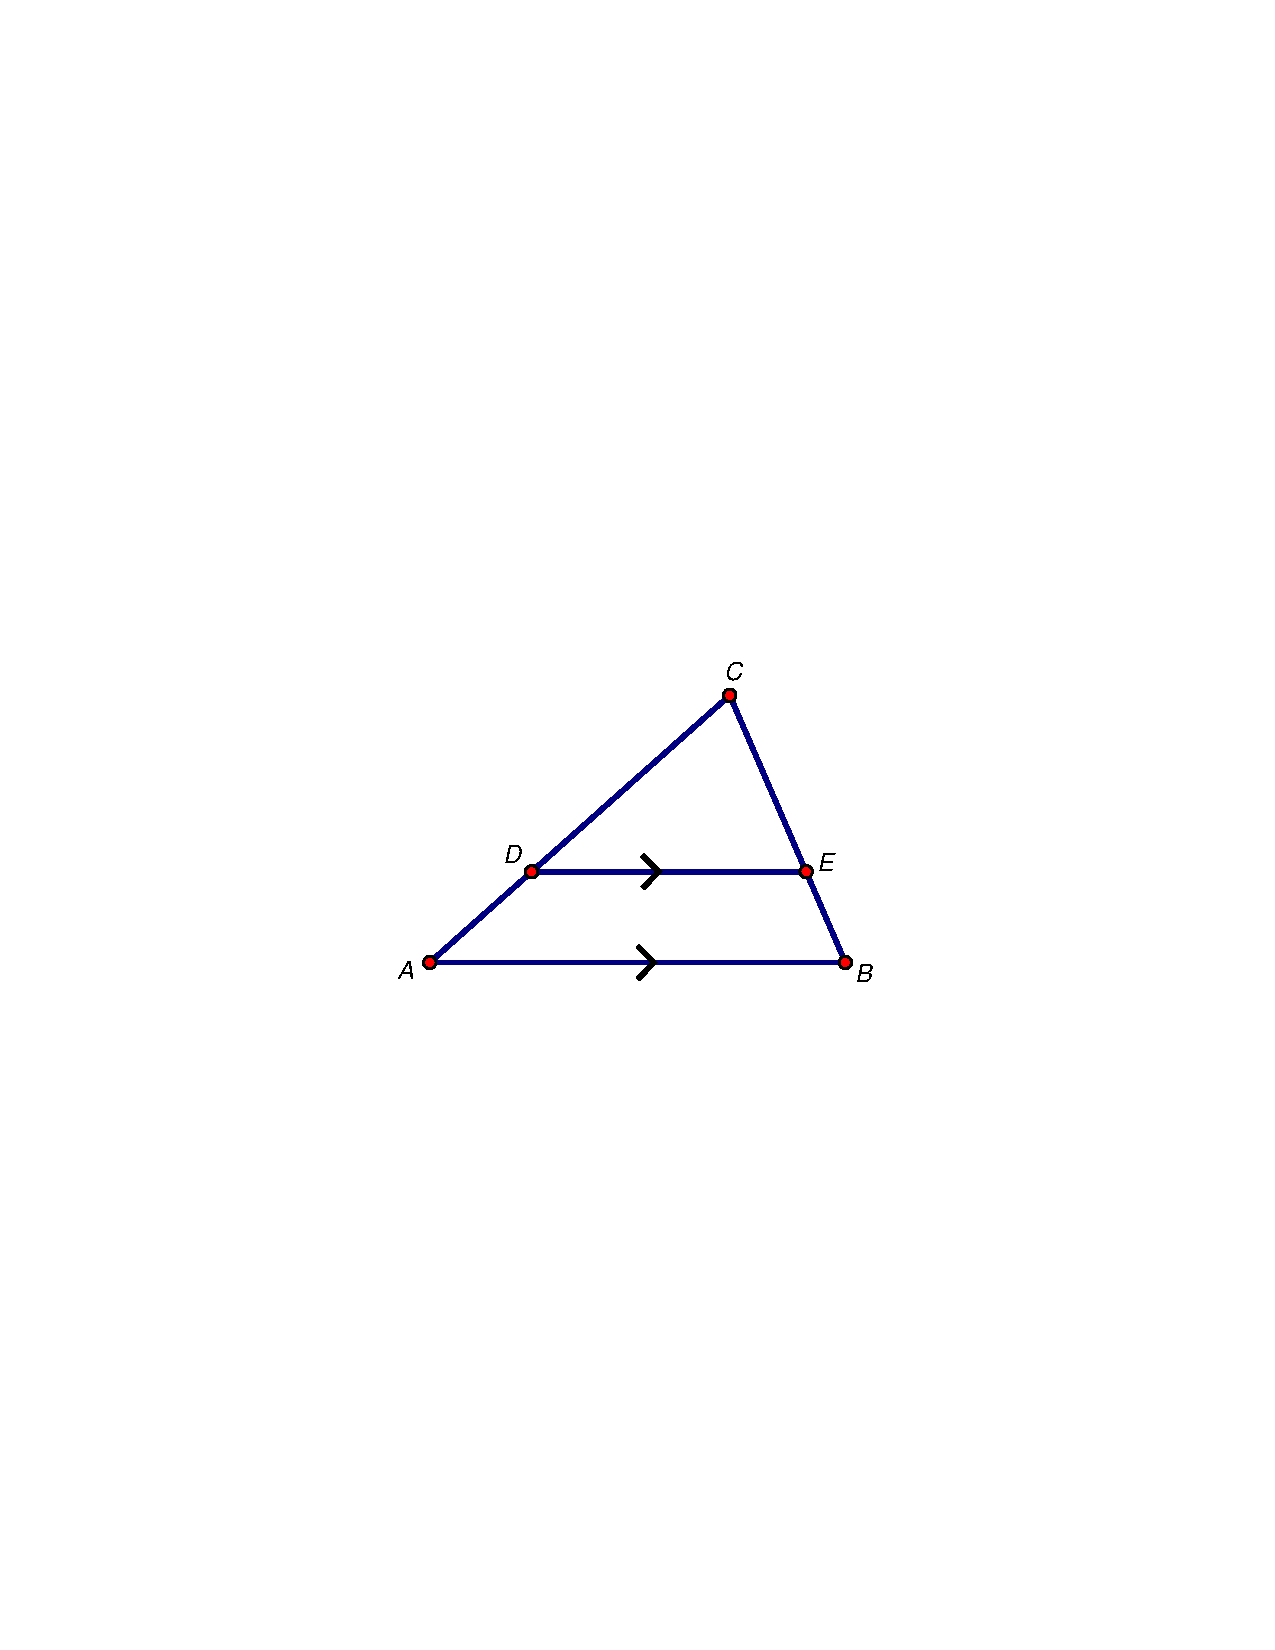
\includegraphics[scale=0.55]{../graphics/Similarity}$$
\begin{enumerate}
\item Using algebra and the Parallel-Side Theorem, you proved that $\frac{AB}{DE}$ is equal to what other ratios?  
%\begin{center}
%$\frac{AB}{DE} = \frac{AC}{DC} =\frac{BC}{EC}$
%\end{center}
\item Explain briefly how the Parallel-Side Theorem implies the AA criterion for triangle similarity.  (Hint: Be sure to use the definition of similarity in terms of basic rigid motions and dilations.)  

\end{enumerate}
\end{prob}

\begin{prob}
The Split-Side Theorem, which is the converse of the Parallel-Side Theorem, is proved in a class activity.   
%(Hint: Using the above figure, draw a line through $D$ and parallel to $\overline{AB}$, 
%and let $X$ be the point where the new line intersects $\overline{BC}$. By the previous results, 
%$\overline{DX}$ divides the sides proportionally. Then argue that $E$ and $X$ must be the same point.)
\begin{enumerate}
\item State the Split-Side Theorem.   (You need not prove it.)
\item Use the Split-Side Theorem to justify the following properties of a dilation given by a center and a scale factor:
\begin{enumerate}
\item A dilation takes a line not passing through the center of the dilation to a parallel line, and leaves a line passing through the center unchanged.
\item The dilation of a line segment is longer or shorter in the ratio given by the scale factor.
\end{enumerate}
\item Explain briefly how the Split-Side Theorem establishes the SAS criterion for triangle similarity.  
\end{enumerate}
\end{prob}
%
%\begin{prob}
%Circles, chords, and areas. Find similar triangles in the figure below in order to establish a relationship among the lengths $AX$, $BX$, $CX$, and $DX$.  Explain your reasoning.
%%\begin{enumerate}
%%\item Find similar triangles in the figure below in order to establish a relationship among the lengths $AX$, $BX$, $CX$, and $DX$.  Explain your reasoning.  
%%%$$\includegraphics[scale=0.45]{Secants}$$
%$$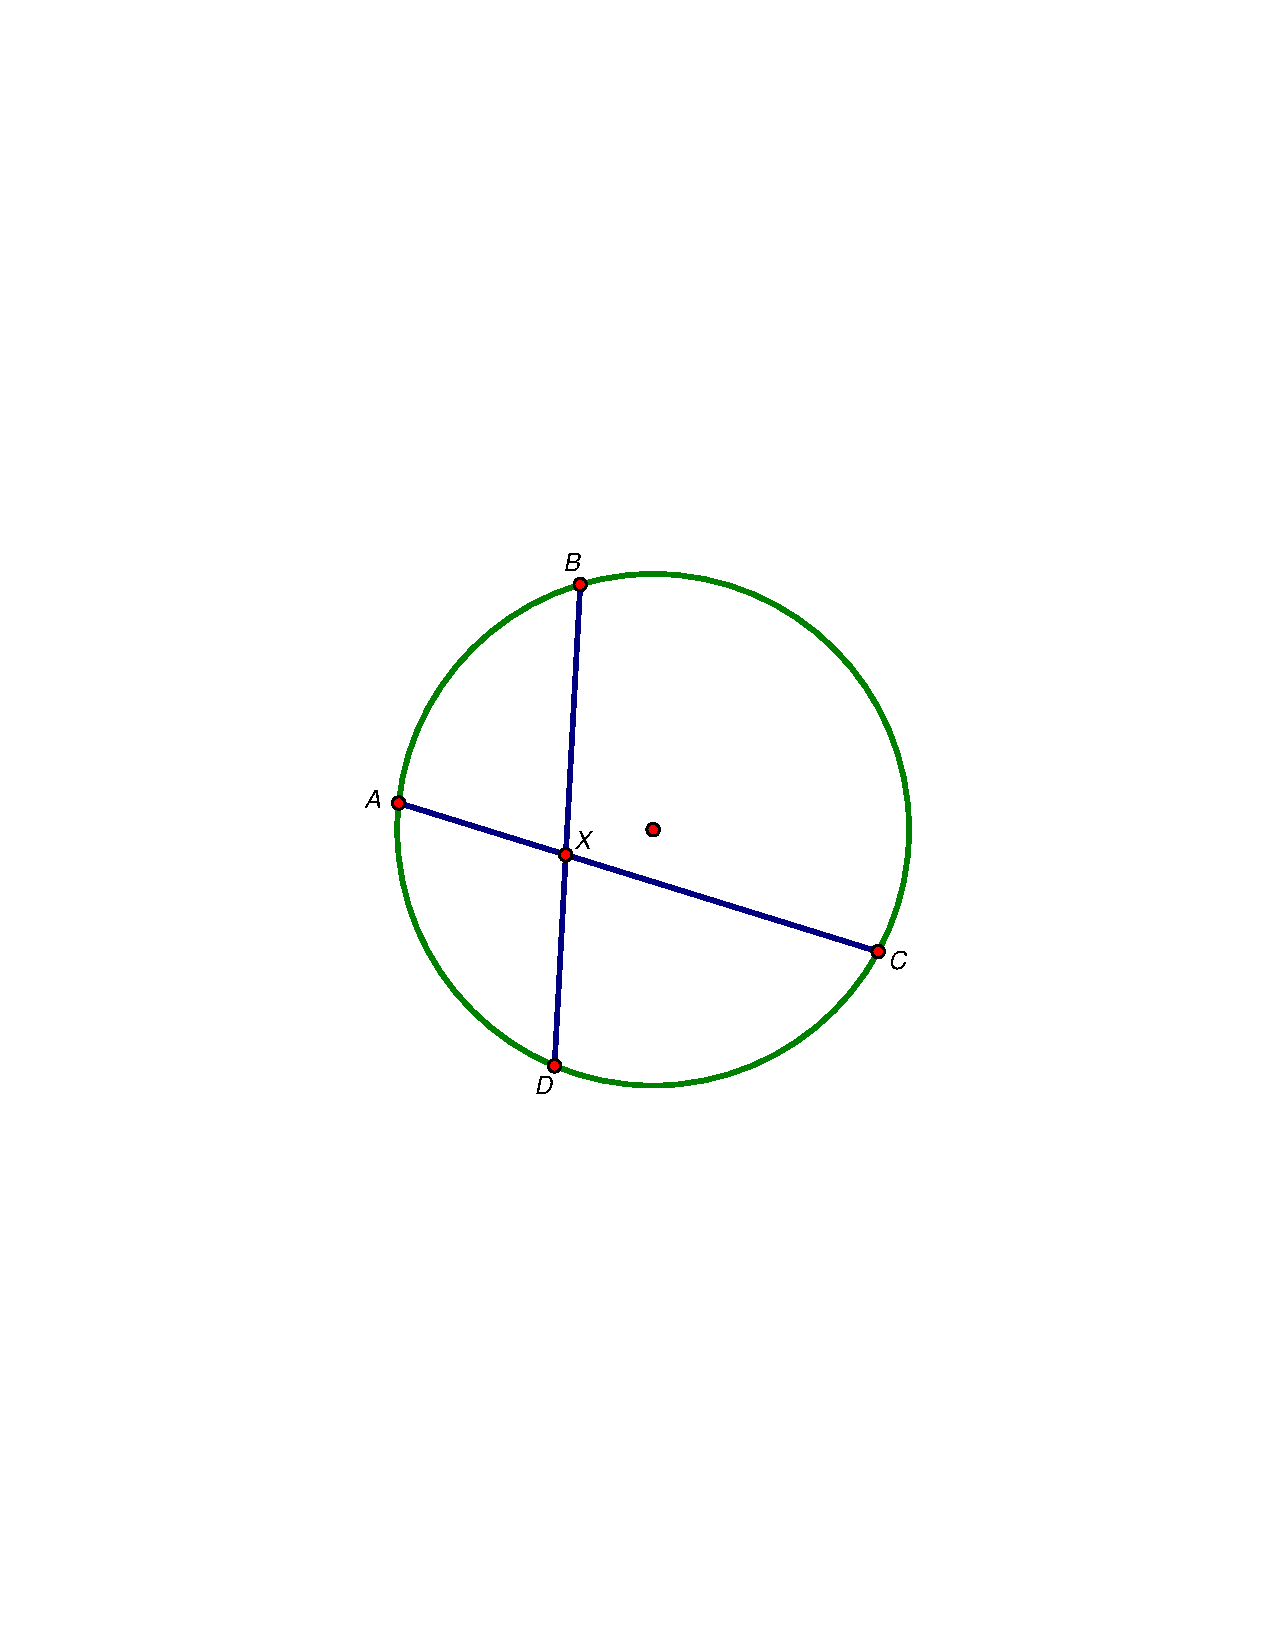
\includegraphics[scale=0.6]{../graphics/CircleChords}$$
%%\item Suppose you are given a rectangle with sides of length $a$ and $b$ (and hence area $ab$).  Suppose you are also given a separate segment of length $c$.  Use your result from part (a) to describe how to construct a rectangle with sides $c$ and $x$ so that it has the same area as the rectangle with sides $a$ and $b$. 
%%\end{enumerate}
%\end{prob}
%


\begin{prob}
Felicia and Wesley are neighbors.  The common boundary between their properties consists of two line segments, as shown below.  
$$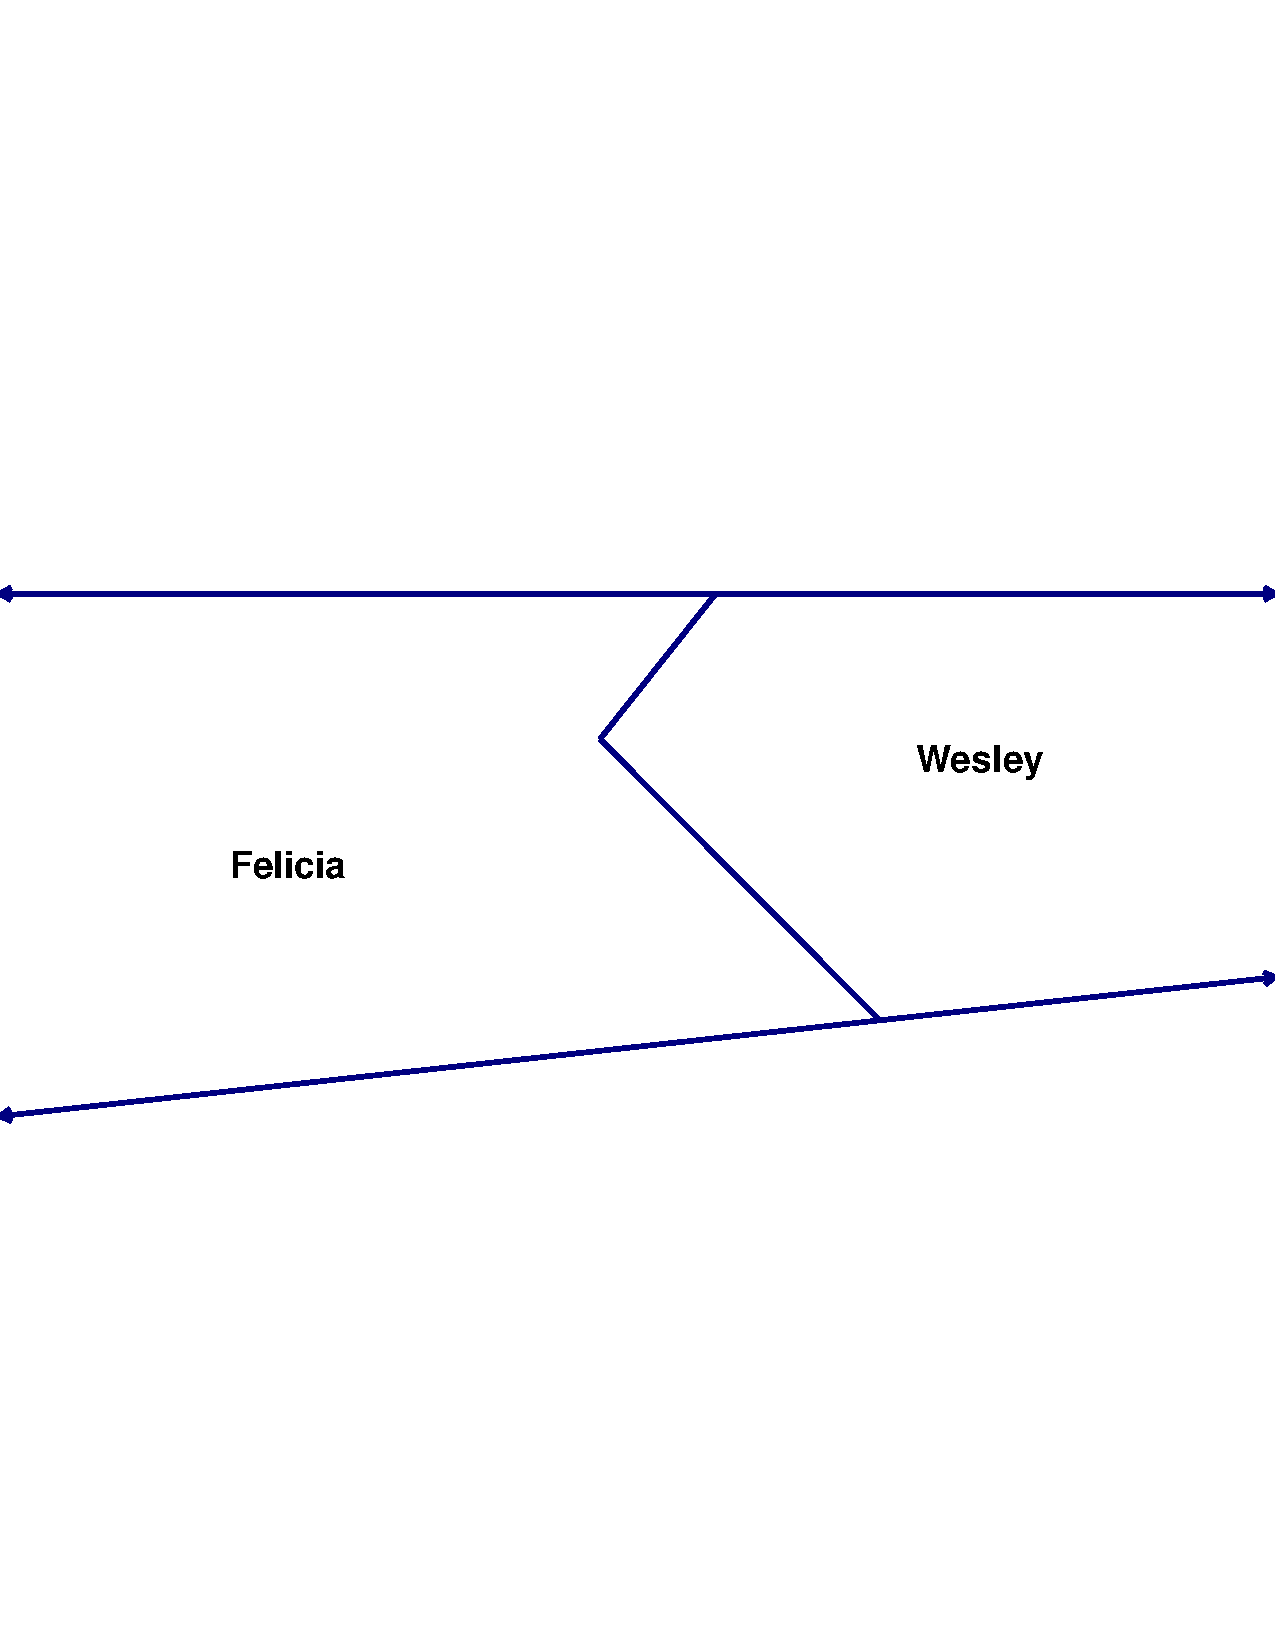
\includegraphics[scale=0.35]{../graphics/TIMSS}$$
They would prefer their common boundary to be a single straight segment.  How might they change their boundary so that they 
each have the same area as they have now?  
\end{prob}

\begin{prob}
Below is a figure that illustrates part of Euclid's proof of the Pythagorean Theorem.  You may assume the following: 
\begin{itemize}
\item All  angles that appear to be right angles are indeed right.
\item $FB=BA$ and $BD=BC$. 
\item $\triangle ABD \cong \triangle FBC$.  
\end{itemize}
\[
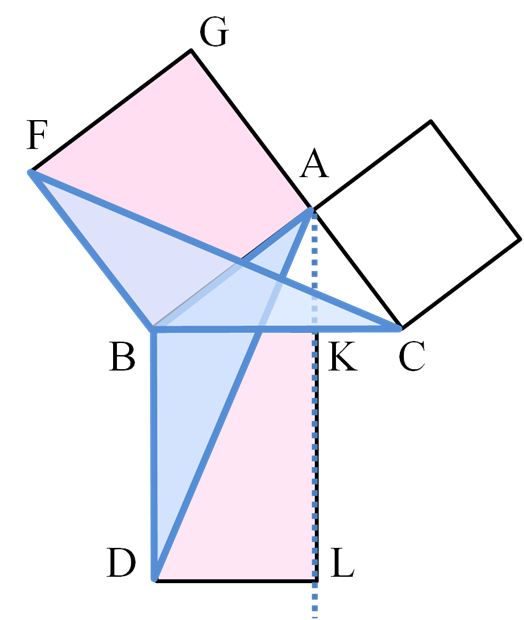
\includegraphics[scale=0.23]{../graphics/Euclid_Pythagorean_theorem3.PNG}
\]
\begin{enumerate}
\item Why is the area of $\triangle KBD$ (not drawn) equal to the area of $\triangle ABD$?
\item Why is the area of $\triangle FBC$ equal to the area of $\triangle FBA$ (not drawn)?
\item Explain briefly why the area of rectangle $KBDL$ equal to the area of rectangle $FBAG$.
\item Now explain how to complete the proof of the Pythagorean theorem.  \end{enumerate}
\end{prob}


\begin{prob}
Describe a general (and foolproof) way of demonstrating that any two parabolas are similar.
\end{prob}

\begin{prob}
Prove that for a triangle, the sum of the interior angles is $180^\circ$.
\end{prob}

%\begin{prob}
%Construct a tangent line from a point outside a given circle to the circle.
%\end{prob}
%
%\begin{prob}
%Explain how the formula for the volume of a sphere follows from the formula for the volume of a cone and Cavalieri's Principle.
%\end{prob}
%
\begin{prob}
Give an informal derivation of the relationship between the circumference and area of a circle. 
\end{prob}

\begin{prob}
Given a figure and a rotation of that figure, find the center and angle of rotation.  
\end{prob}

\begin{prob}
In the figure below  $O$ is the center of the circle, $\overline{XY}$ is a diameter, $a = PX$, $b=PY$, and $c=PZ$.  
$$\includegraphics[scale=0.55]{../graphics/means}$$
\begin{enumerate}
\item Show that $c=\sqrt{ab}$.  
\item Use the figure to explain the Arithmetic-Geometric Mean Inequality: $\frac{a+b}{2} \ge \sqrt{ab}$.  
%\item Why is this called the Arithmetic-Geometric Mean Inequality?  
\end{enumerate}
\end{prob}

\begin{prob}
Use a general (non-special) triangle to explain why every triangle is a rep-4-tile.  
Use the same triangle to explain why every triangle tessellates the plane.  Then use your tessellation to explain why every triangle is a rep-$n^2$-tile for any positive integer $n$. 
\end{prob}


\begin{prob}
 Is it correct to say that ``volume is length times width times height''? What must be true about a figure so that the numerical volume can be more easily measured by ``area times height''?
\end{prob}

\begin{prob}
Are there figures for which there is no formula for measuring length, area, and volume?  Explain.  What does your answer to this question imply about the teaching of geometric measurement?
\end{prob}

\begin{prob}
If the perimeter of a rectangle is 20 feet, what is the most one can say about the rectangle's area?  If the perimeter of any simple closed 2-dimensional shape is 20 feet, what is the most anyone can say about its area?
\end{prob}

\begin{prob}
If the surface area of a rectangular prism is 20 square feet, what is the most one can say about the prism's volume?  If the surface area of any simple closed 3-dimensional shape is 20 square feet, what is the most one can say about its volume? 
\end{prob}

\begin{prob}
Why do cute furry animals curl up to stay warm in the winter?  Why are most ugly desert reptiles long and skinny?
\end{prob}

\begin{prob}Simple closed curve A is contained entirely inside simple closed curve B.  
\begin{enumerate}
\item True or False:  The area enclosed by A is less than the area enclosed by B. Explain
\item True or False:  The perimeter of A is less than the perimeter of B. Explain.  
\end{enumerate}
\end{prob}

\begin{prob}
Is it correct to say that ``area is length times width''?  Think about what these three quantities mean.  When would it be correct in the numerical sense and why?  (Make sure you use the meaning of multiplication.)   
\end{prob}

%\begin{prob}
%The apothem of a regular polygon is defined to be the shortest distance from the center of the polygon to an edge.
%\begin{enumerate}
%\item There is a nice relationship between the apothem, perimeter, and area for a regular polygon.  See if you can find it. (Hint:  Split the polygon into congruent triangles from its center and find the area of the polygon in terms of the apothem and perimeter.)  You can assume you know the area of a triangle $=\frac{1}{2}$(Length of Base)(Length of Height).
%\item What does this result say about the area of a circle?  Explain. (Assume you know the circumference of a circle is $2\pi(radius)$.)
%\end{enumerate}
%\end{prob}


\begin{prob}
Convert 25 yards to meters (and 25 meters to yards) using ``2.54 cm in each inch'' as the only Metric-English unit conversion.  Now convert 25 square yards to square meters and 25 square meters to square yards.  Do the same with cubic yards and cubic meters.
\end{prob}

\begin{prob}
In track and field, 1600 meters is often called the ``one mile,'' but this is not exactly correct.  Is 1600 meters longer or shorter than one mile?  By how much?  
\end{prob}


%\begin{prob}
%Write an equation of the line through $(2,4)$ parallel to $5x-3y=1$.  
%Now write an equation of the line through $(x_1,y_1)$ parallel to $ax+by=c$. 
%\end{prob}
%
%\begin{prob}
%Write an equation of the line through $(2,4)$ perpendicular to $5x-3y=1$.  
%Now write an equation of the line through $(x_1,y_1)$ perpendicular to $ax+by=c$. 
%\end{prob}
%
%\begin{prob}
%Intersections of lines.  
%\begin{enumerate}
%\item Find the intersection of the lines $2x-3y=4$ and $3x-5y=3$.  
%\item Find the intersection of the lines $2x-3y=4$ and $-4x+6y=-8$.
%\item Find the intersection of the lines $2x-3y=4$ and $-4x+6y=5$.
%\item How might you have predicted in advance how many solutions to expect for each previous system of equations?
%\item Use algebra to help explain why lines intersect in zero, one, or infinitely many points.  (You know this geometrically, of course.  Here you demonstrate how algebra gives the same result.)  Indicate clearly the algebraic conditions
%for which you get zero, one, or infinitely many points.  
%\end{enumerate}
%\end{prob}
%
%\begin{prob}
%Suppose you have a rectangle with vertices at $(0,0)$, $(a,0)$,
%$(a,b)$ and $(0,b)$. Use algebra to prove that the diagonals have the
%same length.
%\end{prob}

%\begin{prob} 
%Concurrency of angle bisectors. 
%\begin{enumerate}
%\item For an arbitrary triangle, draw carefully to demonstrate that the angle bisectors of a triangle are concurrent at the incenter.   
%\item Prove that the angle bisectors of a triangle are concurrent.  (Hint:  You may use the result, proved in lecture, that the points on an angle bisector are exactly those that are equidistant from the sides of the angles.)  
%\end{enumerate}
%\end{prob} 

%\begin{prob}
%Explain how the ASA congruence criterion follows from the definition of congruence in terms of rigid motions. Be sure to indicate, using the two given angles and the included side, why the sequence of rigid motions guarantees triangle congruence.
%\end{prob}

%Other review
% * Multiplication is not necessarily scaling--unless it is dilation
%
% * Use of cavalieri's principle 
% * Volume as Area of base times height.
% * Stacking cubic units covering the base. 


